\chapter{盒子模型与布局模型}

\section{元素分类}

\subsection{我要独占一行——块级元素}

在HTML中\lstinline|<div>|、\lstinline|<p>|、\lstinline|<h1>|、\lstinline|<form>|、\lstinline|<ul>|、\lstinline|<li>|等都是块级元素。每个块级元素都从新的一行开始,并且其后的元素也另起一行。块级元素的高度、宽度、行高遗迹顶和底边距都可以设置,宽度在不设定的情况下,是它本身父容器的100\%(和父元素的宽度一致)。

\begin{lstlisting}[style=htmlcssjs, title=块级元素]
<!DOCTYPE html>
<html lang="en">
<head>
    <meta charset="UTF-8">
    <title>块级元素</title>
</head>
<body>
    <div>这是一个div标签</div>
    <p>这是一个p标签</p>
    <h1>这是一个h1标签</h1>
</body>
</html>
\end{lstlisting}

通过设置\lstinline|display: block|可以将元素显示为块级元素。

\subsection{我要和你站一起——内联元素}

在HTML中,\lstinline|<span>|、\lstinline|<a>|、\lstinline|<label>|、\lstinline|<strong>|、\lstinline|<em>|等都是内联元素(行内元素)。内联元素和其它元素都在一行上,元素的高度、宽度及顶部和底部编剧不可设置,元素的宽度就是它包含的文字或图片的宽度,不可改变。 \\

块级元素也可以设置\lstinline|display: inline|将元素设置为内联元素。

\begin{lstlisting}[style=htmlcssjs, title=内联元素与块级元素转换]
<!DOCTYPE html>
<html lang="en">
<head>
    <meta charset="UTF-8">
    <title>内联元素与块级元素转换</title>
    <style type="text/css">
        a {
            display: block;
        }

        div {
            display: inline;
        }
    </style>
</head>
<body>
    <a>我要变成块级元素</a>
    <a>我也要变成块级元素</a>

    <div>我要变成内联元素</div>
    <div>我也要变成内联元素</div>
</body>
</html>
\end{lstlisting}

\subsection{我还要占个大位置——内联块状元素}

内联块状元素就是同时具备内联元素和块级元素的特点。内联块状元素的特点是和其它元素都在一行上,但元素的高度、宽度、行高以及顶和底边距都可以设置。 \\

通过设置\lstinline|display: inline-block|就可以将元素设置为内联块状元素。如\lstinline|<img>|、\lstinline|<input>|就是这种内联块状标签。

\newpage

\section{盒子模型}

\subsection{盒子模型}

盒子模型包含4个部分:

\begin{enumerate}
    \item 外边距(margin)
    \item 外边框(border)
    \item 内边距(padding)
    \item 内容(content)
\end{enumerate}

\begin{figure}[H]
    \centering
    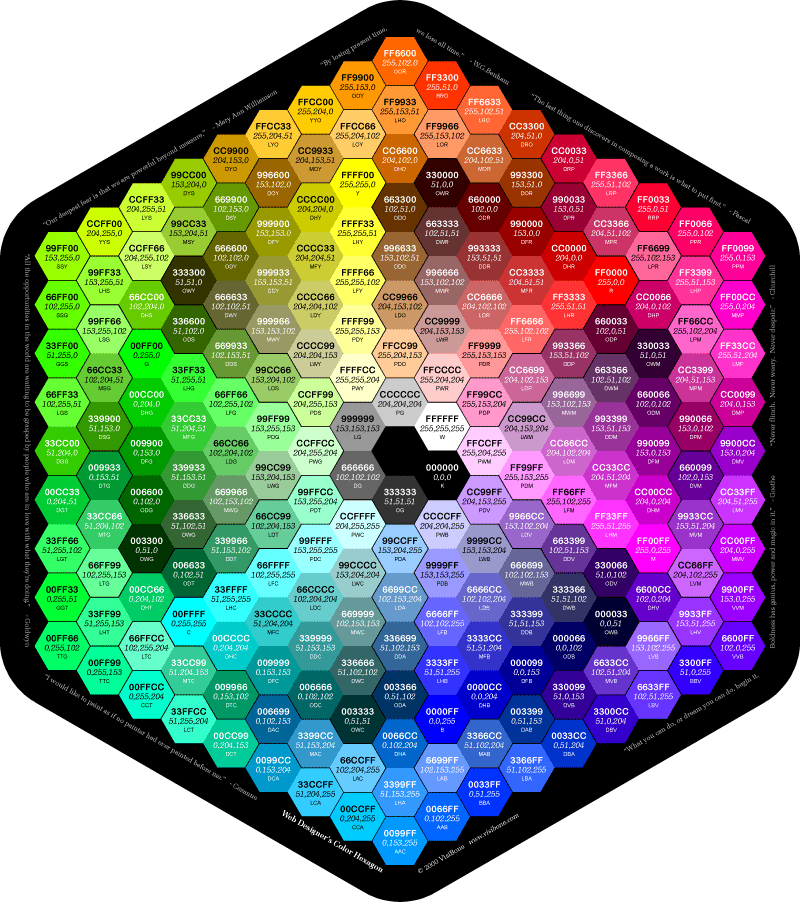
\includegraphics[scale=0.7]{img/C8/8-2/1.png}
\end{figure}

盒模型的宽度和高度和平常所说的物体的宽度和高度的理解是不一样的,CSS内定义的宽和高,指的是盒模型中内容的宽和高。 \\

元素实际的宽度(盒子的宽度) = 左外边距 + 左边框 + 左内边距 + 内容宽度 + 右内边距 + 右边框 + 右外边距 \\

\begin{figure}[H]
    \centering
    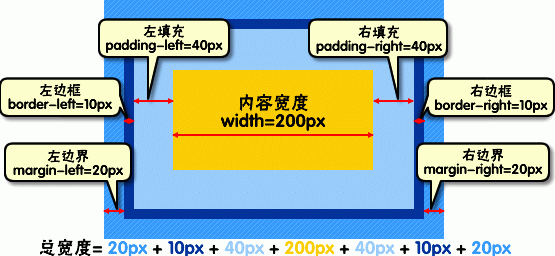
\includegraphics[]{img/C8/8-2/2.png}
\end{figure}

\subsection{外边框(Border)}

盒子模型的外边框可以设置粗细、样式和颜色:

